\documentclass[11pt]{iopart}
\usepackage{fullpage}

\usepackage{iopams,graphicx,color}
\usepackage{setstack}
\usepackage[pdftex,breaklinks=true,bookmarks=false,colorlinks=true,citecolor=violet,urlcolor=blue,linkcolor=red]{hyperref}
\usepackage{tikz}

\newcommand{\psm}{p_{\sigma,\mu}}

\begin{document}
 
\title[Correlations and entanglement in the 2D RVB wave function]{Correlations and entanglement in the two-dimensional resonating valence bond wave-function}
 
\author{Jean-Marie St\'ephan$^1$, Hyejin Ju$^2$, Paul Fendley$^1$, Matthew B. Hastings$^3$ and Roger G. Melko$^4$}

\address{$^1$ Physics Department, University of Virginia, Charlottesville, VA 22904-4714}

\address{$^2$ Department of Physics, University of California, Santa Barbara, CA, 93106-9530}

\address{$^3$ Microsoft Research, Station Q, CNSI Building, University of California, Santa Barbara, CA, 93106-9530}

\address{$^4$ Department of Physics and Astronomy, University of Waterloo, Ontario, N2L 3G1, Canada}

\eads{\mailto{jean-marie.stephan@virginia.edu}, \mailto{ju@physics.ucsb.edu}}

\date{\today}
\submitto{NJP}
\begin{abstract}
 We study correlations and entanglement in the $SU(N)$ nearest-neighbor RVB wave function.
\end{abstract}
\maketitle




\section{Introduction}
\subsection{Resonating valence bond wave function}
\paragraph{}\textcolor{red}{\bf [History of RVB, Anderson, Quantum spin liquids, \ldots]}

\paragraph{}


The nearest-neighbor resonating valence-bond wavefunction on the square lattice has striking if somewhat schizophrenic behavior. Correlators in this state can be written in terms of the correlators of a two-dimensional classical loop model where loops longer than length two have a weight of $4$ per loop. A spin-spin correlator corresponds to having a strand of loop end at the sites of the spins \cite{Doucot}. Such a correlator is exponentially decaying  whenever the weight per loop is greater than 2 \cite{Nienhuis}.  Moreover, extensive numerics indicate \cite{RVB1,RVB2} have not found any  spin order. In this sense, the spins are ``deconfined'' and this state perhaps represents a sort of spin liquid.

On the other hand, the RVB wave function bears an obvious similarity to the ground state of the
 the quantum dimer model (QDM)\cite{RokhsarKivelson}: a nearest-neighbor spin-slnglet in the RVB wave function can be thought of as a dimer connecting the two sites. In the QDM one forgets the underlying spins: the only degrees of freedom in the quantum dimer model are the nearest-neighbor dimers. Different dimer configurations are orthogonal in the QDM, but  not in the RVB case. One very convenient feature of the QDM is that  correlators in its ground state here can be computed exactly even on the lattice, because they are exactly those of the two-dimensional classical dimer model. This can be mapped on to a free fermion problem (i.e.\ computing the Pfaffian of a specific matrix), and their asymptotic behavior easily obtained \cite{Kasteleyn, Fisher}. On the square lattice, dimer-dimer correlators were long ago shown to be algebraically decaying \cite{FisherStephenson}.

This similarity makes it plausible the the correlator of two ``dimers'' (i.e. two nearest-neighbor spin singles) in the RVB case will behave in a similar fashion to the dimer-dimer correlator in the QDM. This expectation is further supported by the fact that one can interpolate between the two wave functions, either by studying an $SU(N)$ version as described below, or by dressing the lattice itself \cite{RMS}, and there is no evidence for any phase transition. Such algebraic decay of   ``dimer-dimer'' correlations  in the RVB state was convincingly demonstrated numerically
\cite{RVB1,RVB2}:
 \begin{equation}
  C_{dd}(\vec{r}_1,\vec{r}_2) \sim \left|\vec{r}_1-\vec{r}_2\right|^{-\alpha}
 \end{equation}
The exponent was found to be close to $\alpha \approx 1.2$. This is an even weaker falloff than in the QDM, where $\alpha_D=2$ \cite{FisherStephenson}. By the theorem of \cite{Hastings_thm}, algebraic decay of local operators in a two-dimensional ground state requires that any local Hamiltonian with this ground state be gapless. Thus the QDM at its RK point is gapless, as is the Hamiltonian of Ref.~\cite{Cano}, whose ground-state is exactly the RVB state. 

%\paragraph{}

A very useful fact about the classical dimer model is that long-distance properties of the dimers are described by a free bosonic field theory. This can be seen by either by bosonizing the fermions, or by rewriting the dimers in terms of an integer ``height'' degree of freedom \cite{Heights_1,Heights_2,Henley}. Either approach implies that the scaling limit of the classical dimer model is a free scalar field $h(x,y)$ with euclidean action
 \begin{equation}\label{eq:free_field}
  S=\frac{\kappa}{4\pi}\int \left(\nabla h\right)^2 dx dy,
 \end{equation}
 where $h$ is compactified on a circle of radius $1$: $h=h+2\pi$. The coupling $\kappa$ is often known as the ``stiffness''. Such a field theory description is also known as a ``Coulomb Gas'', and is an example of a two-dimensional conformal field theory, the free boson CFT, with central charge $c=1$ \cite{Nienhuis,Ginsparg}. It is ubiquitous in two-dimensional statistical models, as well as in condensed matter, where it describes Luttinger liquids.   This model is critical but not Lorentz-invariant, with dynamical critical exponent $z=2$.  The dimers are viewed as elementary electric charges, and the dimer-dimer exponent in the ground state is given in general by
\begin{equation}
 \alpha=\frac{1}{\kappa}.
\end{equation}
This yields the stiffness for the dimer model $\kappa_D=1/2$. Elementary magnetic charges can also identified with monomers, and the corresponding exponent describing their two-point function is given by $\beta=\kappa$, so $\beta_D=1/2$.
Once the stiffness fixed to its right value, Eq.~(\ref{eq:free_field}) describes all the universal properties of the dimer model.
In this framework the quantum dimer model can also be written as in terms of a free scalar field in the 2+1 dimensional ``quantum Lifshitz'' model \cite{Henley,Fradkin_dimers}. This is an example of a conformal quantum critical point, where the equal-time correlators of a 2d {\em quantum} model are those of a 2d conformal field theory.

\paragraph{} Given the substantial difference in the exponents, the RVB wave function is obviously not identical to that for dimers. However, Ref.~\cite{RVB2} found however that long-distance properties of the $SU(2)$ RVB wave function are still described by a Coulomb gas, albeit with a different stiffness, yielding different exponents. This was shown by computing numerically several universal quantities, including the dimer-dimer and monomer-monomer exponent. With appropriate identification of the operators, each yields a independent value for the the stiffness, $\kappa_{RVB}\approx .83$. The numerics gave approximately the same value of the stiffness for each, providing strong evidence that the Coulomb gas description applies to correlators of {\em spin singlets} in the RVB wave function. The $SU(2)$ RVB wave function, just like its QDM counterpart, therefore enjoys a very special property. Although it is a $2$d quantum system, equal-time ground-state properties of spin-singlets correspond to a 2d conformal field theory\cite{QuantumLifshitz} and 
Notice that while the height representation can be understood from simple lattice arguments in the dimer model, no such intuitive argument exists for the RVB state. 

It is purpose of this paper to explore these critical properties of the RVB state.


\paragraph{}To help understand the emergence of the height field description, it is useful to generalize this study to the $SU(N)$ case. Any correlator calculated in the $N\to \infty$ limit reduces to the same correlation in the dimer model. Such a correspondence can actually be pushed further: Ref.~\cite{Damle} defined a cluster expansion of the RVB ``loop gas''\cite{Sutherland_loops} in terms of interacting dimers in the large $N$ limit. Remarkably, one recovers to first non trivial order the model studied in \cite{Alet_dimers1,Alet_dimers2}, for which the height description is more natural. The $\alpha$ exponent extrapolated to $N=2$ turned out to be in good agreement with the previous numerical studies\cite{RVB1,RVB2}.
\paragraph{}
All this results motivate us to look in details at the $SU(N)$ RVB wave function. Our objective is twofold: 
\begin{itemize}
 \item First, we want to confirm the short range spin order of the spin correlation, as well as the criticality of the dimer correlations. Our approach is more direct, and uses Monte-Carlo simulations in the valence bond basis. In particular, we determine the spin correlation length as well as the dimer exponent up to $N=5$. We expect this exponent to interpolate between the $SU(2)$ and dimer exponent. 
 \item Most of the studies so far -- with \cite{Ju2012,Poilblanc} as a notable exceptions -- have focused only on correlation functions. It however important to look at more complicated obvservables, to check wether universal properties of this wave function survive. We will focus here on the R\'enyi entanglement entropy, defined through a bipartition of the quantum system $A\cup B$:
 \begin{equation}
  S_n=\frac{1}{1-n}\ln \left({\rm Tr}\, \rho_A^n\right)\quad ,\quad \rho_A={\rm Tr}_B\, |\psi\rangle \langle \psi|.
 \end{equation}
The case $n=2$ is particularly interesting, because the entropy can then be efficiently simulated in the valence bond basis, as the expectation value of a Swap operator\cite{swap}. We will here extend the results already reported in \cite{Ju2012} for $SU(2)$, and discuss in more details how to extract the universal features  of this entropy in general.
\end{itemize}
\subsection{Geometry}
\paragraph{}In this paper, we study the $SU(N)$ square lattice RVB wave function in a \emph{finite} torus geometry, as shown in Fig.~\ref{fig:torus}. The torus has dimensions $L_x$ and $L_y$. Physical results obviously depend on the aspect ratio of the cylinder. We encode this in a parameter, the modulus $\tau$ of the torus:
\begin{equation}
 \tau=i\frac{L_y}{L_x}
\end{equation}
The imaginary number is there for purely technical reasons, as it allows to make contact with standard results of conformal field theory. Most of the numerical studies will be performed for the most simple and natural case $L_y=L_x$, but we expect our results to generalize to any aspect ratio. Except for explicit mention of the contrary we will therefore assume $L_x=L_y=L$ in the numerical simulations.
\paragraph{}
To study the entanglement we cut the system in two cylindrical subsystems $A$ and $B$, as shown in Fig.~\ref{fig:torus}. Subsystem $A$ (emphasized in bold blue) is a cylinder of circumference $L_x$ and height $\ell_y=y L_y$, while $B$ is a cylinder of circumference $L_x=L$ and height $L_y-\ell_y=(1-y)L_y$. We call
\begin{equation}
 y=\frac{\ell_y}{L_y}
\end{equation}
the ``subsystem ratio''. 
We are interested in the scaling behavior of the entropy with $L$, while keeping both ratios $y$ and $\tau$ finite. 
\begin{figure}[ht]
 \begin{center}
  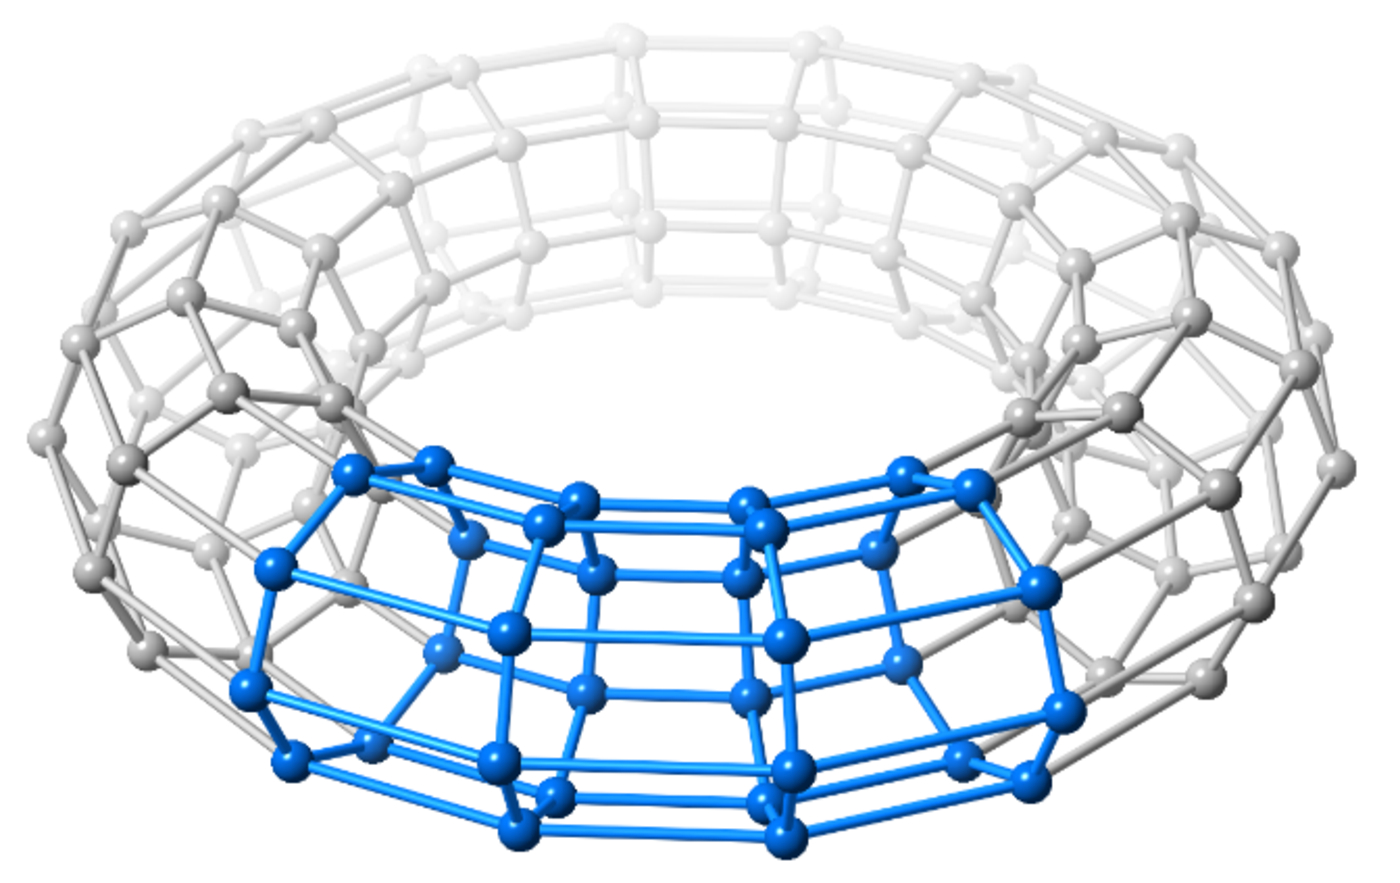
\includegraphics[width=7cm,angle=-90]{./figures/16x8b.pdf}
  \end{center}
  \caption{Example of torus geometry studied in this paper, with $L_x=8$ and $L_y=16$. We are interested in correlations as well as entanglement. For the latter one needs to cut the system in two parts $A$ and $B$. Here subsystem $A$ is a cylinder of heigth $\ell_y=4$, and is drawn in bold blue. Subsystem $B$ is a cylinder of height $\ell_y=L_y-\ell_y=12$. Notice that $L_x$ and $L_y$ have been intertwined, compared to Ref.~\cite{Ju2012}.}
\label{fig:torus}
 \end{figure}
\paragraph{}
 It is well known that the R\'enyi entanglement entropy of such quantum systems exhibits an area law\cite{ALreview}:
\begin{equation}
 S_n(L,y,\tau)= a_{n} L+s_{n}(y,\tau)+\mathcal{O}(1/L)
\end{equation}
Since the boundary between $A$ and $B$ is smooth and assuming a Coulomb gas description, we expect no subleading logarithmic corrections\cite{Hsu09}. The first subleading term should be a universal constant $s_n(y,\tau)$, which depends only on the two aspect ratios for a given universality class. In particular, we are interested in the dependence of $s_n$ on the subsystem ratio $y$. At this stage it is important to notice that although $a_n$ is non-universal -- and therefore depends on the specifics of the lattice model -- this area law term should \emph{not} depend on the two aspect ratios. This simple fact has an important practical consequence: one can read off the $y$ (or $\tau$) dependence of $s_n(y,\tau)$ by just looking at the numerical data $S_n(L,y,\tau)$ for sufficiently big $L$. We will use this method throughout the paper, therefore sidestepping any  (possibly difficult in practice) fitting procedure.    
 \subsection{Outline}
 The paper is organized as follows:
 \begin{itemize}
 \item In Sec.~\ref{sec:basics} we recall some basic properties of the $SU(N)$ nearest-neighbors wave function on the square lattice. In particular, we discuss the well known connection to a classical loop gas\cite{Sutherland_loops}, and how to perform Monte-Carlo simulations in the valence-bond basis.
 \item Correlations are studied in Sec.~\ref{sec:correlations}. We show that while the spin-spin correlations decay exponentially, the dimer-dimer correlations are critical. The exponent approaches $\alpha=2$ as $N$ increases, and agrees well with the large $N$ computation of \cite{Damle}. We also present further evidence of the underlying Coulomb-Gas.
 \item We then focus on the entanglement, starting in Sec.~\ref{sec:dimers_entanglement} with a somewhat detailed description of the simplest dimer case. While the entanglement properties of quantum dimer wave functions are now relatively well understood, the finite torus has been left aside until now. We show how some of the previous  results can be generalized for our purposes. 
 \item Finally, Sec.~\ref{sec:rvb_entanglement} presents numerical simulations of entanglement for the $SU(N)$ RVB wave function, and tries to provide physical intuition, as well as a field-theoretical description of the results. In particular, we find striking similarities with the QDM behavior, and therefore strong evidence of universal behavior. 
\end{itemize}
\section{Some basic properties of the $SU(N)$ RVB wave function.}
\label{sec:basics}
\subsection{Definition}
Let us start with a two-dimensional lattice, which will be the square lattice for us. An $SU(N)$ singlet between sites $i$ and $j$ is given by
\begin{equation}
\label{eq:rvb}
  [i,j]=\frac{1}{\sqrt{2S+1}}\sum_{m\in \{-S,-S+1,\ldots,S\}}^{}(-1)^{m-S}\,|m\rangle_i \otimes |-m\rangle_j,
 \end{equation}
 with $N=2S+1$. When $i$ and $j$ are nearest neighbors,
 such a singlet can be viewed as a ``dimer'', occupying the link between sites $i$ and $j$. Suppose now the number of sites is even:
\begin{equation}
 L_x L_y=2M\quad,\quad M \in \mathbb{N}.
\end{equation}
Just as in the classical dimer model, one can define a dimer configuration ${\cal C}$, which is a covering of the lattice by dimers $(i_\alpha,j_\alpha)$ such that each site be occupied by one dimer and one dimer only: ${\cal C}=\{(i_1,j_1),(i_2,j_2),\ldots ,(i_{M},j_{M})\}$. 
A valence bond state is a tensor product of these dimer states
\begin{equation}
\label{eq:vbbasis}
 |V_{\cal C}\rangle=[i_1,j_1] \otimes [i_2,j_2] \otimes \ldots \otimes [i_{M},j_{M}]
\end{equation}
The nearest-neighbor RVB wave function is then defined as an equally weighted superposition of these valence-bond states:
 \begin{equation}
  | {\rm RVB}\rangle=\sum_{\cal C} |V_{\cal C}\rangle,
 \end{equation}
where the sum runs over all possible dimer configurations of the lattice. Notice that the number of dimer coverings increase exponentially with the system size. Asymptotically one has\cite{Kasteleyn}
\begin{equation}
 Z=\sum_{\mathcal{C}}1\sim (1.79162\ldots)^M
\end{equation}
\subsection{Non orthogonality and simulations}
One of the main features of valence bond states is that they are not orthogonal
\begin{equation}
\label{eq:overlap}
 \langle V_{\cal C}|V_{{\cal C}^\prime}\rangle=\pm (2S+1)^{{\cal L}-M},
\end{equation}
where ${\cal L}$ is the number of loops in the transition graph formed by superimposing the two dimer configurations ${\cal C}$ and ${\cal C}^\prime$. Notice that ${\cal L}$ can be at most $M$, and this happens only when all the loops are trivially flat, i.e when the two dimer configurations are identical. We have however
\begin{equation}
 \langle V_{\cal C}|V_{{\cal C}^\prime}\rangle=\delta_{{\cal C},{\cal C}^\prime}
 \end{equation}
 in the limit $S\to \infty$ (or equivalently $N \to \infty$). As a result, any correlation calculated in the limit $N\to \infty$ will be identical to that in the corresponding dimer model. It is however important to stress that this argument only holds at the level of correlation functions.
\paragraph{}
\textcolor{blue}{\bf [Add explanations about QMC simulations, windings, and other stuff.]}

%
%%
%%%
%Hyejin's changes

\subsection{Numerics}

In our Monte Carlo simulation, we employ a loop sampling algorithm that moves through the ensemble of states by creating a defect at some lattice site and propagating it through the system until the defect reaches its initial point and closes the loop~\cite{sandvik2010loop}. Our algorithm is very similar to the $SU(2)$ updates used in ~\cite{RVB2}; however, we need to generalize to account for $SU(N)$ RVB wavefunctions. At each Monte Carlo step, we form the transition graphs to compute Eq.(~\ref{eq:overlap}). Using this transition graph, we sample the value of $m \equiv S^z$ at each site. This gives us a larger set of constraints in that the loop can only update within a compatible $m$ as defined in Eq.(~\ref{eq:rvb}). Then, the case of $N=2$ is equivalent to having two independent subset that can only be updated within each subset. For a larger $N$, the number of updates that one can make becomes much smaller, and the error bars become much harder to converge, which can be cured by using a smarter update that satisfies detailed balance to allow the simulation to make more updates.

In our valence bond basis Monte Carlo simulation, we compute various correlation functions, namely the spin-spin and the dimer-dimer correlations. The matrix elements, first derived in~\cite{beach2006some} and generalized in~\cite{beach2009n} for $SU(N)$ spins, are shown below, using the notation $(ij)_L$ for two sites $i,j$ in the same loop in the transition graph and $(i)_L(j)_L$ for sites not in the same loop~\cite{RVB2}.
\[ 
\displaystyle
\frac{\langle V_\mathcal{C} | \mathbf{S}_i \cdot \mathbf{S}_j | V_{\mathcal{C}'} \rangle}{\langle V_\mathcal{C} | V_{\mathcal{C}'} \rangle} = \left\{ \begin{array}{ccc}
0 & (i)_L (j)_L\\
\epsilon_{ij} \, S (S+1) & (ij)_L   \end{array}. \right.
\] 
Here, $\epsilon_{ij} = 1$ if $(i,j)$ are on the same sublattice and $\epsilon_{ij} = -1$ if they are on different sublattices.
We measure \textit{parallel} nearest neighbor dimer-dimer correlations, i.e.
\[ 
\displaystyle
\frac{\langle V_\mathcal{C} | \left( \mathbf{S}_i \cdot \mathbf{S}_j \right) \left( \mathbf{S}_k \cdot \mathbf{S}_l  \right) | V_{\mathcal{C}'} \rangle}{\langle V_\mathcal{C} | V_{\mathcal{C}'} \rangle} = \left\{ \begin{array}{ccc}
\frac{1}{3} S^2 (S+1)^2 & (ik)_L (jl)_L, \,(il)_L (jk)_L\\
S^2 (S+1)^2 & (ij)_L (kl)_L \end{array}, \right.
\] 
and $0$ otherwise. Because we are measuring parallel dimer-dimer correlations, we take $j = i + \hat{e}_\alpha, \, l = k + \hat{e}_\alpha$ and $k = i + \hat{e}_\beta$, where $\alpha,\beta = x, y, \, \alpha \neq \beta$.

%\cite{beach2009n} (sun)
%\cite{beach2006some} (formal valence bond MC paper)
%\cite{sandvik2010loop} (loop updates for vb basis)





%End of Hyejin's changes
%%%
%%
%






 \section{Correlations}
In this section we compute numerically the spin-spin correlations, as well as the dimer-dimer correlations, on a torus of size $L_x=L_y=L=64$. For simplicity we look at correlations along the $x$ direction, the two spins or dimer being separated by a distance $\ell_x$ (so that $\ell_y=0$). For convenience we will sometimes express the results in terms of the reduced parameter
\begin{equation}
 x=\frac{\ell_x}{L_x}.
\end{equation}
\label{sec:correlations}
\subsection{Spin-spin correlations}
\begin{figure}[ht]
 \begin{center}
  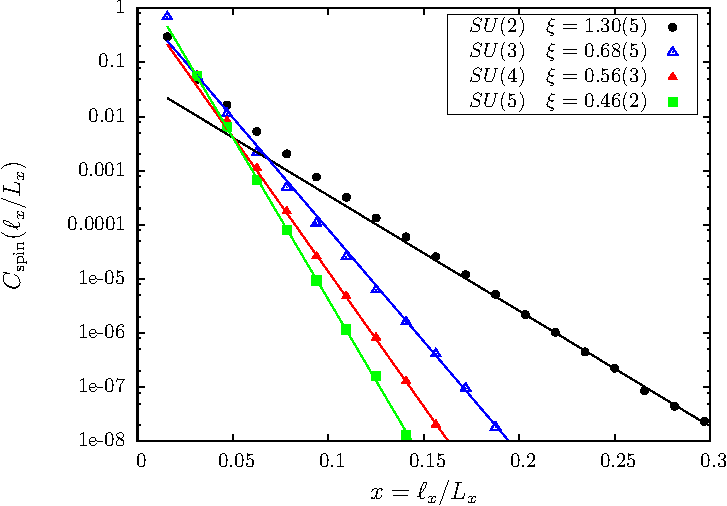
\includegraphics{./figures/spin_corr.pdf}
 \end{center}
\caption{Spin-spin correlation function on the torus. They decay exponentially, with an exponent that diminishes with $N$. We have $\xi(N=2)=1.30(5)$ (compatible with \cite{RVB1}) and the new $\xi(N=3)=0.68(5)$, $\xi(N=4)=0.56(3)$ and $\xi(N=5)=0.46(2)$.}
\label{fig:corr_su2}
\end{figure}
Let us first look at the spin correlations. As is shown in Fig.~\ref{fig:corr_su2}, they decay exponentially
\begin{equation}
 \langle S(0)S(\ell_x) \rangle \sim \exp \left(-\frac{\ell_x}{\xi}\right)
\end{equation}
with a finite correlation length $\xi$. This is well known\cite{Doucot,RVB1} for the $SU(2)$, and our data generalizes these previous results. This short-range N\'eel order supports a quantum spin-liquid  behavior. We also observe that $\xi$ decreases with $N$, compatible with the intuition that the RVB state becomes more and more spin-disordered as $N$ increases.
\subsection{Dimer-Dimer correlations}
Let us now look at the more interesting dimer-dimer correlations. The connected dimer-dimer correlation function has been recently shown to decay algebraically in Refs.~\cite{RVB1} and \cite{RVB2} for $SU(2)$. One has to leading order \textcolor{blue}{\bf [give more details]}
\begin{equation}\label{eq:decay}
 D_{||}(\ell) \sim (\ell/L)^{-\alpha},
\end{equation}
in the limit $1\ll \ell \ll L$.
The exponent is approximately $\alpha_2\simeq 1.2$. We extend here these results to the $SU(N)$ case, focusing on longitudinal correlation with an odd distance between the two dimers\footnote{\textcolor{red}{\bf [give a few more details, and also maybe the even-distance correlation. Discuss subleading corrections.]}}, and in the $W=(0,0)$ sector. Since we have
\begin{equation}
 \lim_{N \to \infty} \alpha_N=\alpha_{\rm dimers}=2,
\end{equation}
it is reasonable to expect that the exponent will interpolate smoothly between the two values. 
\begin{figure}[ht]
 \begin{center}
  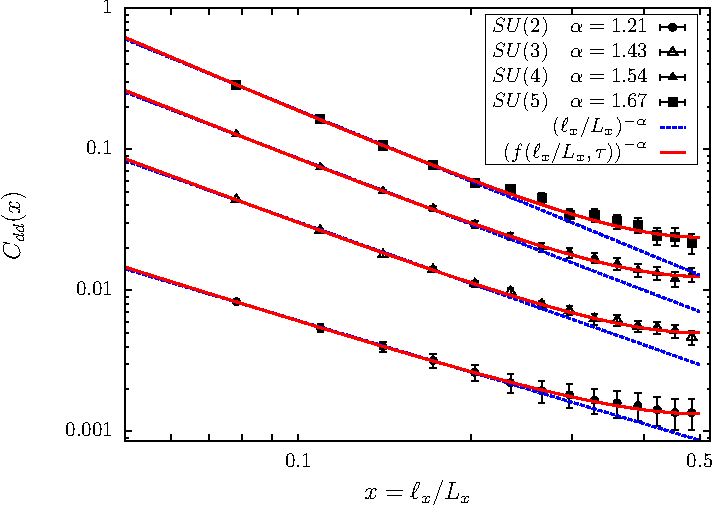
\includegraphics{./figures/corr_su2.pdf}
 \end{center}
\caption{Dimer-Dimer correlations on the $64 \times 64$ torus for $N=2,3,4,5$. Dashed blue lines is a linear fit to Eq.~(\ref{eq:decay}), in the ``linear regime'' $\ell_x \simeq 5,\ldots,15$. We also performed a fit to the conformal scaling (Eq.~\ref{eq:cft_fit}) in the same region (red solid lines). Such a fit reproduces all the data quite well.}
\label{fig:corr_su2_dimers}
\end{figure}
\paragraph{}Our numerical results are shown in Fig.~\ref{fig:corr_su2_dimers}. For each $N$ we extract the leading exponent by a fit (solid blue lines in Fig.~\ref{fig:corr_su2_dimers}) to Eq.~(\ref{eq:decay}) in the regime $1\ll \ell \ll L$. We find $\alpha_2=1.21(2)$, $\alpha_3=1.43(3)$, $\alpha_4=1.54(3)$, $\alpha_4=1.67(6)$. Notice that as $N$ gets larger, it becomes more and more difficult  to converge the Monte-Carlo data in a finite time, which implies a loss of precision on the corresponding exponent. 
\paragraph{}This values turn out to be in good agreement with an alternative computation by Damle {\it et al}\,\cite{Damle} in the large $N$ limit. In this reference, the authors define a cluster expansion of the loop model corresponding to RVB in terms of a classical interacting dimer model. To first nontrivial order, this model is exactly the one studied by Alet {\it et al}\,\cite{Alet_dimers1,Alet_dimers2}, and this allows to use their Monte-Carlo results. In addition to the already reported $\alpha_2\simeq 1.22$, this approach yields\footnote{Notice that we determined these exponents just from looking at Fig.~26 in \cite{Alet_dimers2}. In their notations,  $X_2=\alpha/2$ and $W=1+1/N$.} $\alpha_3 \simeq 1.4$, $\alpha_4 \simeq 1.52$, and $\alpha_5\simeq 1.6$. Our numerical results therefore confirm that the higher order interacting terms only have a small influence on the critical exponent. 
\paragraph{}
Since we are performing simulations on a torus, it is tempting to relax the constraint $\ell \ll L$, and therefore to take into account its finiteness in the fit. While the two-point function on a torus cannot be determined from the sole requirement of conformal invariance, it is known for a $c=1$ Luttinger liquid CFT\cite{BigYellowBook}. Therefore, assuming the underlying height model, the Eq.~(\ref{eq:decay}) is modified in the following way:
\begin{equation}\label{eq:cft_fit}
 D_{||}(\ell_x)\sim f(\ell_x/L_x,\tau)^{-\alpha},
\end{equation}
with $\ell_x \gg 1$. $f$ is a universal function of the two dimensionless ratios $\ell_x/L_x$ and $\tau =i L_y/L_x$ and can be expressed in terms of a Jacobi Theta function (\ref{sec:CFT_Jacobi}). We have 
\begin{equation}
 f(\ell/L_x,\tau)=\sum_{n=0}^{\infty}(-1)^n \sin \left[(2n+1)\pi \ell/L_x\right]e^{-\pi n(n+1)(L_y/L_x)}
\end{equation}
Notice that while this function reduces to $f(x,\tau)=\sin(\pi \ell/L_x)$ in the limit of a thin torus ($L_y/L_x \gg 1$), the latter is still an almost perfect approximation for $L_y/L_x=1$. Performing the fits to Eq.~(\ref{eq:cft_fit}) in the same region $1\ll \ell \ll L_x$ as before (red solid curve in Fig.~\ref{fig:corr_su2_dimers}), we observe that the data reproduces very well the CFT prediction, even the upturn when $\ell$ is of order $L_x$. This is additional evidence for the underlying height model. However, the exponents determined this way are slightly larger. For example we find $\alpha_2\simeq 1.26$. This small discrepancy with the previous $SU(2)$ results\cite{RVB1,RVB2} could possibly be resolved studying larger systems, but could also be an indication that previously claimed error bars were slightly underestimated.  
  \section{Entanglement in the quantum dimer wave function}
\label{sec:dimers_entanglement}
Although the critical exponents of the (quantum) dimer model have been known for a long time, the study of entanglement in such types of wave functions started only recently\cite{Moore06,Hsu09,Misguich,Oshikawa,Zaletel,Stephan11}. Most of the work so far has focused on semi-infinite geometries such as the infinite cylinder\cite{Hsu09,Misguich,Oshikawa} or the infinite band\cite{Moore06,Zaletel,Stephan11}, but the finite torus we are interested in has been so far neglected.
\paragraph{}
We show here how to extend the previous results to the torus geometry and extract the universal shape of the R\'enyi entropy, in the spirit of \cite{Ju2012}. This will allow us to gain some crucial understanding before studying the RVB states, as the connection between dimers and (boundary) conformal field theory is much better understood. 
\subsection{Entanglement entropy as a Shannon entropy}
The orthogonality of the dimer configuration in the quantum language allows for huge technical simplifications. As was shown in Ref.~\cite{Misguich}, the entanglement entropy can be expressed as a classical Shannon entropy. We give here only a brief summary of the results, and refer to \cite{Misguich} for the details.
\paragraph{} Let us cut our torus in two subsystems $A$ and $B$, as is shown for example in Fig.~\ref{fig:bipartition}.
\begin{figure}[ht]
\begin{center}
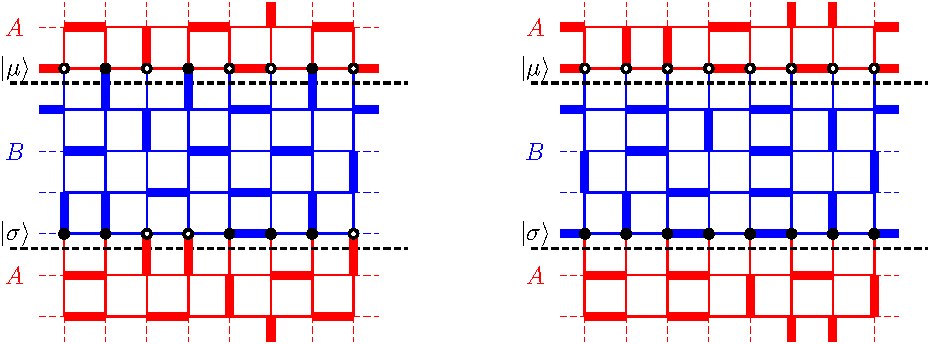
\includegraphics{./figures/bipartition.pdf}
\end{center}
\caption{Bipartition of the $8\times 8$ torus. Links in subsystem $A$ (resp. $B$) are shown in red (resp. blue). The two boundaries between $A$ and $B$ are emphasized by thick dashed lines. Links crossing the lower boundary are in $A$, whereas those crossing the upper boundary are in $B$. Sites closest to the boundary are called ``boundary sites''. We attach an $\uparrow$ (resp. $\downarrow$) virtual spin to a boundary site occupied by a dimer in $B$ (resp. $A$) and represent it by a black (resp. white) filled circle. Each boundary configuration has probability $p_{\sigma,\mu}$. \emph{Left}: Example of dimer configuration compatible with $|\sigma\rangle=|\!\uparrow\uparrow\downarrow\downarrow\uparrow\uparrow\uparrow\downarrow\rangle$ and $|\mu\rangle=|\!\downarrow\uparrow\downarrow\uparrow\downarrow\downarrow\uparrow\downarrow\rangle$. \emph{Right}: Example of dimer configuration compatible with the most likely boundary configuration $|\sigma\rangle=|\!\uparrow\uparrow\uparrow\uparrow\uparrow\uparrow
\uparrow\uparrow\rangle$ and $|\mu\rangle=|\!\downarrow\downarrow\downarrow
\downarrow\downarrow\downarrow\downarrow\downarrow\rangle$, where no dimers are crossing the boundary.}
\label{fig:bipartition}
\end{figure}
The main difference with \cite{Misguich} is that there are two boundaries here, but the the same arguments apply. The von Neumann entropy can be recast as a classical Shannon entropy
\begin{equation}
 S=-\sum_{\sigma,\mu} p_{\sigma,\mu} \ln p_{\sigma,\mu}
\end{equation}
The $p_{\sigma,\mu}$ are the probabilities of a given boundary configuration $|\sigma\rangle$,$|\mu\rangle$ between $A$ and $B$, defined in Fig.~\ref{fig:bipartition}. They are given by
\begin{equation}
 \psm=\frac{Z_{\sigma,\mu}}{Z},
\end{equation}
where $Z_{\sigma,\mu}$ is the number of dimer configurations compatible with the boundary configuration $|\sigma\rangle,|\mu\rangle$. $Z$ is the number of dimer coverings on the whole torus. The $\psm$ are nothing but the eigenvalues of the reduced density matrix, and the mapping therefore allows to calculate  any R\'enyi entanglement entropy as
\begin{equation}
 S_n=\frac{1}{1-n}\ln \left(\sum_{\sigma,\mu}[\psm]^n\right).
\end{equation}
As explained in \ref{sec:lgv}, each probability can be expressed as a product of 2 determinants of size $\sim L/2$, and computed numerically in a time of order $\approx L^3$. Using translationnal symmetry along the $x$ axis as well as the conservation of winding numbers, we are able to compute any R\'enyi entropy up to machine precision in a time of order $L^{3/2}\times 4^L$.
\subsection{Boundary phase transition}
We now discuss the behavior of the R\'enyi entropy as a function of $n$, and in particular the boundary phase transition emphasized in \cite{Stephan11}. At long distance universal properties are described by the free compactified field with action
 \begin{equation}\label{eq:free_field_bis}
  S_\kappa[h]=\frac{\kappa}{4\pi}\int \left(\nabla h\right)^2 dx dy,
 \end{equation}
However, one also has to take into account contributions from irrelevant vertex operators near the boundary:
\begin{equation}
 V_d=\cos \left(d \,h\right).
\end{equation}
with $d$ an integer. If such a term was to dominate, it would lock the height field to a flat configuration with degeneracy $d$. The renormalization group analysis of such operators is standard\cite{Coleman}: $V_d$ is irrelevant as long as $d^2>2\kappa$. This argument is however too naive.  
In the continuum limit the $p_{\sigma,\mu}$ are promoted to configurations of the field $p(\phi)$. The probability to observe the field configuration $\phi$ at the boundary is still gaussian
\begin{equation}
 p(\phi)\propto \exp(-S_{\kappa}[\phi]),
\end{equation}
and raising this probability to the $n-$th power yields
\begin{equation}
 [p(\phi)]^n=\exp(-n S_{\kappa}[\phi])=\exp(-S_{n\kappa}[\phi]).
\end{equation}
Therefore, the system near the boundary effectively feels a stiffness $\kappa^\prime=n\kappa$. As a consequence, if one whishes to compute $S_n$, $V_d$ is irrelevant as long as $d^2>2n\kappa$. This defines two regions, separated by a phase transition. The critical value of $n$ is
\begin{equation}
 n_c=\frac{d_{\rm min}^2}{2\kappa},
\end{equation}
where $d_{\min}$ is the smallest $d$ allowed by the lattice symmetries. On the square lattice $d_{\rm min}=1$ and $\kappa=1/2$, so that the critical value is
\begin{equation}
 n_c=1.
\end{equation}
For $n>n_c$, the field locks onto the minimum of $V_{1}$, and universal contributions to the R\'enyi entropy are dominated by the configuration:
\begin{equation}
 S_{n>n_c}\sim \frac{n}{1-n}\ln (p_{\rm max})
\end{equation}
The configuration with maximum probability corresponds to a cut with no dimer crossing the boundaries between $A$ and $B$. This is a huge technical simplification, as
\begin{equation}\label{eq:pmax}
 p_{\rm max}=\frac{Z_{\rm cyl}(L_x,y L_y)Z_{\rm cyl}(L_x,(1-y)L_y)}{Z_{\rm torus}(L_x,L_y)}
\end{equation}
can be computed exactly on the lattice (see \ref{sec:dimers_exact}), as well as in the continuum limit (see Sec.~\ref{sec:universal_shape}). This make the extension of previous results\cite{Misguich,Stephan11} rather straightforward, as we shall see in the next section. Before going any further, let us make the following remarks:
\begin{itemize}
 \item It should also be possible to extend the quantum dimer results\cite{Misguich,Oshikawa,Zaletel,Stephan11} to finite-size in the region $n<n_c$, using boundary CFT methods. This is certainly an interesting question for future studies, and could also involve subtle issues regarding analytic continuation\footnote{Oshikawa\cite{Oshikawa} has already treated the $y=1/2$ case for the closely related cylinder geometry, using the replica approach $n\in \mathbb{N}$. Similarly to the two interval 1d EE\cite{CCT1,CCT2}, the analytic continuation to real $n$ turns out to be non-trivial.}. It however falls outside the scope of the present paper.
 \item We will present evidence in Sec.~\ref{sec:rvb_entanglement} that the calculation of $S_2$ for RVB is in the phase $n>n_c$. This is our main motivation for a complete study of the quantum dimer case, \emph{after the transition}.
 \item It is important to notice that even though $s_n$ should take an universal form in both phases, the value itself of the critical R\'enyi parameter depends on a degeneracy $d_{\rm min}$, which is non-universal. For example, $d_{\rm min}=2$ for the quantum six-vertex wave function, and $d_{\rm min}=3$ for quantum dimers on the hexagonal lattice. 
 \item The cylinder geometry can obtained by replacing the denominator of Eq.~(\ref{eq:pmax}) by a cylinder partition function. As a consequence, the torus and cylinder geometry should exhibit the same universal shape, \emph{after the transition}.
 \item From the QDM perspective, the R\'enyi entanglement entropy is effectively a simple fidelity\cite{Bipartite_fidelity}:
 \begin{equation}\label{eq:lbf}
  S_{n>n_c}\sim \frac{n}{1-n} \ln \left|\langle A\cup B|A\otimes B\rangle\right|^2,
 \end{equation}
where $|A\cup B\rangle$ is the ground-state wave function of the whole system. $|A\otimes B\rangle$ is the ground-state wave function where all interactions between $A$ and $B$ have been switched off, a tensor product of the two ground-state wave functions in $A$ and $B$. Furthermore, Eq.~(\ref{eq:lbf}) even becomes exact on the lattice when $n\to \infty$.
  \item The entanglement spectrum $\{E_{\sigma,\mu}\}=\{-\ln p_{\sigma,\mu}\}$ of such types of wave functions does not any gapless excitations, compared to the more studied Quantum Hall case \cite{HaldaneLi}. We have therefore an example of a system that is \emph{gapless} in the bulk, but \emph{gapped} at the edge. 
  %\textcolor{red}{\bf [Entanglement spectrum comments. Bulk gapless boundary gapped (for us) vs Bulk gapped boundary gapless (Haldane-Li Quantum Hall).]}
\end{itemize}
\subsection{Numerical results}
We present here some numerical simulations to emphasize the influence of the phase transition we previously discussed. The results are summarized in Fig.~\ref{fig:ee_d_torus}. 
\begin{figure}[htbp]
 \begin{center}
 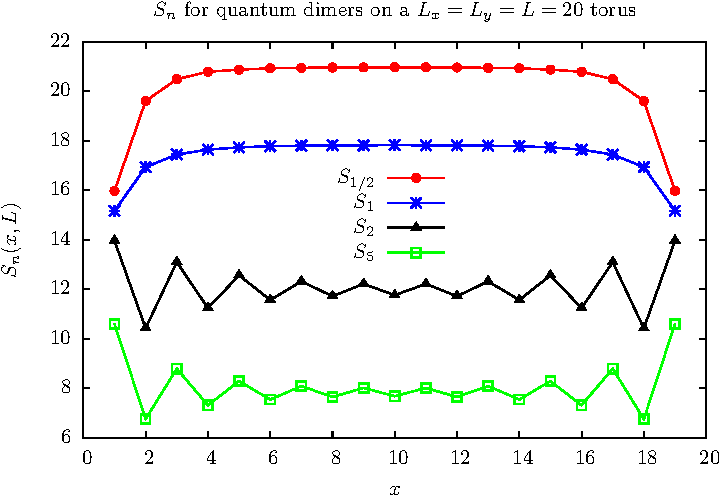
\includegraphics[width=10cm]{./figures/ee_d_torus.pdf}
 \end{center}
\caption{R\'enyi entanglement entropy for quantum dimers on the square lattice in the torus geometry. Here $L_x=L_y=20$, and we present data for $S_{1/2}$, $S_1$, $S_2$ and $S_5$. The even-odd effect is a signature of the ``locked phase'' for $n>1$. In this phase the even-odd effect is proportionnal to $n/(n-1)$, and therefore slightly diminishes with $n$. We compute it exactly in \ref{sec:universal_shape}}
\label{fig:ee_d_torus}
\end{figure}
The entropy exhibits strikingly different behaviors in the two regimes. In the ``replica phase'' $n \leq 1$, the curves are relatively flat. In the thermodynamic limit we expect it to go to a universal function, which may be computed from boundary CFT. As already stated, this however falls outside the scope of the present paper. In the locked phase we observe a strong even-odd effect, which we explain in the next section.  
\subsection{Even odd effect and universal shape after the transition}
\label{sec:universal_shape}
For $n>1$, we expect the universal subleading constant to be given by
\begin{equation}\label{eq:shape_general}
 s_n=\frac{n}{1-n}\ln \left(\frac{{\cal Z}_{\rm cyl}(y\tau) {\cal Z}_{\rm cyl}((1-y)\tau)}{{\cal Z}_{\rm torus}(\tau)}\right),
\end{equation}
where the $\mathcal{Z}$ are the universal CFT partition functions. For the free boson CFT, they depend on the geometry (cylinder, torus, \ldots), on the aspect ratio $\tau=iL_y/L_x$, on the stiffness, and also on the \emph{boundary conditions}. These partition functions can be identified from the lattice model, as the constant term in the asymptotic expansion of the lattice partition functions:
\begin{equation}
 \ln Z= a L^2+b L+\ln \mathcal{Z}+O(1/L).
\end{equation}
Let us focus on the cylinders, which encode the $y$-dependence we are interested in. The boundary conditions at the top and bottom correspond to flat configurations for the microscopic heights, which are expected to renormalize to a Dirichlet boundary condition ($D$) for the height field $h$. Such a partition function is well known within CFT\cite{FSW}:
\begin{equation}\label{eq:cyl_dd}
 \mathcal{Z}_{\rm cyl}^{DD}(\tau)=\frac{\theta_3(2\tau)}{\eta(2\tau)},
\end{equation}
and can even be derived from the exact lattice partition function, see \ref{sec:dimers_exact}. It turns out this reasoning is only valid when the height of the cylinder is even. As is shown in Fig.~\ref{fig:height_shift}, when $L_y$ is odd the heights at the top are slightly shifted compared to the bottom. 
\begin{figure}[ht]
 \begin{center}
 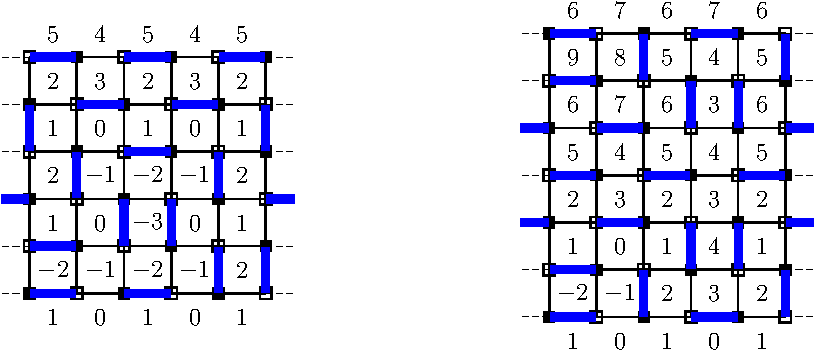
\includegraphics{./figures/shift.pdf}
 \end{center}
\caption{Illustration of the height shift between the upper and lower boundaries in the odd case. The mapping to microscopic heights goes as follows. Turning counterclockwise around a site of the even (resp. odd) sublattice represented by black squares (resp. white squares) the height picks $-3$ (resp. $+3$) if it crosses a dimer, $+1$ (resp. $-1$) otherwise. All heights are expressed in units of $\pi/2$. 
 \emph{Left:} Even $L_y$ case. The coarse-grained heigth difference between top and bottom is $\Delta h=\langle h_{\rm top}\rangle-\langle h_{\rm bottom}\rangle=(\pi/2)(9/2-1/2)=2\pi$. It is easy to check that $\Delta h=2\pi w$, $w\in \mathbb{Z}$ holds for all dimer configurations. \emph{Right:} Odd $L_y$ case. We have $\Delta h=(\pi/2)(13/2-1/2)=3\pi$. It is also easy to check that in general $\Delta h=2\pi (w+1/2)$, $w\in \mathbb{Z}$.}
\label{fig:height_shift}
\end{figure}
\paragraph{}
More precisely, the corse-grained height difference between top and bottom is given by
\begin{equation}
 \Delta h =h_{\rm top}-h_{\rm bottom}=2\pi (w+a)\quad,\quad w \in \mathbb{Z},
\end{equation}
where $a=0$ for even $L_y$ and $a=1/2$ for odd $L_y$. 
Such a small shift has a tremendous impact in the continuum limit. The partition function may be computed using the standard decoupling of the action into an oscillator part, and a classical part, which is subject to compactification. See for example \cite{EggertAffleck,FSW,BigYellowBook} for more details. 
The partition function for general $a$ is given by
\begin{equation}
 \mathcal{Z}_{\rm cyl}^{DD^{(a)}}=\frac{1}{\eta(-1/2\tau)}\sum_{w \in \mathcal{Z}}\exp \left[-\kappa \pi\frac{L_x}{L_y} (w+a)^2\right].
\end{equation}
In the even case $a=0$, one recovers, upon setting $\kappa=1/2$ and after modular transformation (\ref{sec:modular}), the Eq.~(\ref{eq:cyl_dd}). For $a=1/2$, the odd partition function is given by 
\begin{equation}
 \mathcal{Z}_{\rm cyl}^{DD^\prime}(\tau)=\frac{\theta_4(2\tau)}{\eta(2\tau)}.
\end{equation}
We finally remark that such a strong even-odd effect has been subject to several studies in the dimer model\cite{Ferdinand,Dimers_all,Ruelledimers}, although it has to our knowledge never been interpreted in the context of the height mapping. Plugging these results in Eq.~(\ref{eq:shape_general}), and using the torus partition funtion\cite{BigYellowBook} also given in the appendix, one finally gets
\begin{eqnarray}\label{eq:cft_prediction}
 s_n^{\rm (even)}(y,\tau)&=&\frac{n}{1-n}\ln \left(\frac{\eta(\tau)^2}{\theta_3(2\tau)\theta_3(\tau/2)}\times\frac{\theta_3(2y \tau)\theta_3(2(1-y)\tau)}{\eta(2y\tau)\eta(2(1-y)\tau)}\right)\\
 s_n^{\rm (odd)}(y,\tau)&=&\frac{n}{1-n}\ln \left(\frac{\eta(\tau)^2}{\theta_3(2\tau)\theta_3(\tau/2)}\times\frac{\theta_4(2y \tau)\theta_4(2(1-y)\tau)}{\eta(2y\tau)\eta(2(1-y)\tau)}\right)
\end{eqnarray}
Fig.~\ref{fig:dimers_shape} shows a numerical test of the universal shape Eq.~(\ref{eq:cft_prediction}) for quantum dimers, for two different aspect ratios $L_y/L_x=1$ and $L_y/L_x=2$.  
\begin{figure}[ht]
\begin{center}
 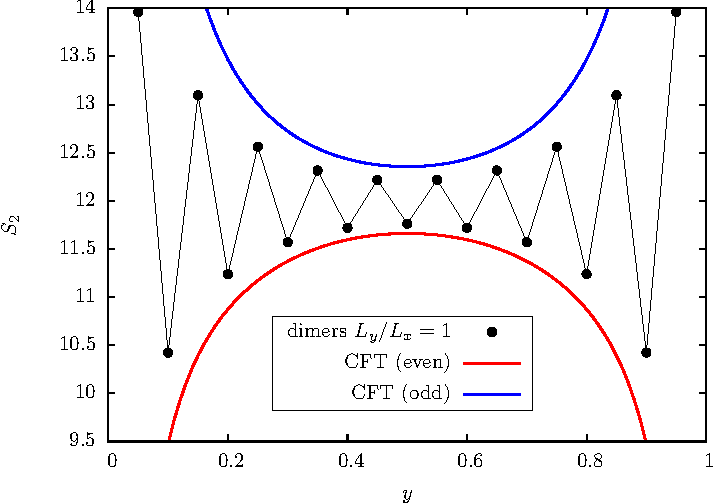
\includegraphics[width=8cm]{./figures/dimers_shape.pdf}
 \end{center}
 \caption{Numerical results for the second R\'enyi entropy $S_2$ as a function of the subsystem-ratio $y$ for $L_x=20$ and two torus aspect ratios $L_y/L_x=1,2$. The CFT prediction is given by Eq.~(\ref{eq:cft_prediction}) up to a \emph{single} constant representing the area law term. For $L_y\gg L_x$, $S_2$ goes exponentially fast to a perfectly flat curve, and the even-odd effect disappears.}
 \label{fig:dimers_shape}
\end{figure}
\paragraph{}
Several interesting observations can be made:
\begin{itemize}
 \item The universal shape we obtain bears strong resemblance to the numerical results of Ref.~\cite{Ju2012}, strengthening a posteriori the author's claim at universality.  
 \item The curves get flatter and flatter when increasing $L_y/L_x$: one recovers this way the more studied infinite torus limit, where $s_n$ becomes independent on $y$. It could have been tempting to expect the result to be similar to the celebrated 1d quantum result\cite{CC} $S_n\propto \ln\sin (\pi y)$ in the infinite torus limit. This is clearly not the case, and one can easily check that the corresponding quasi-1d system would be massive, and therefore cannot exhibit the conformal scaling. 
 \item The even-odd effect also disappears in this limit. Our finite-size geometry therefore exhibits a richer behavior than its infinite counterpart.
 \item Notice also that the agreement with the numerics, while fair, is not that good. We attribute this small mismatch to strong finite-size effects. We discuss them further in Sec.~\ref{sec:exact}.
\end{itemize}
\subsection{The exactly solvable $n=\infty$ limit}
\label{sec:exact}
To illustrate the slowness of the convergence, we also perform simulations in the exactly solvable case $S_\infty=-\ln p_{\rm max}$ (Eq.~\ref{eq:pmax}), where the agreement between CFT and the lattice can be made rigorous. $s_{\infty}$ is obtained by taking the $n\to \infty$ limit in Eq.~(\ref{eq:cft_prediction}). 
As an additional test one can also compute $s_\infty$ in the $W=(0,0)$ winding sector. The calculation is performed in the appendix. The result reads:
\begin{eqnarray}\label{eq:cft_w0}
 s_\infty^{\rm (even)}&=&-\ln \left(\frac{\eta(\tau)^2\theta_3(2y(1-y)\tau)}{\eta(2y\tau)\eta(2(1-y)\tau)}\right)\\
 s_\infty^{\rm (odd)}&=&-\ln \left(\frac{\eta(2\tau)^2\theta_4(2y(1-y)\tau)}{\eta(2y\tau)\eta(2(1-y)\tau)}\right)
\end{eqnarray}
Notice that even in this sector there are still contributions coming from the compactified nature of the height field. This can be explained by the fact that while the total winding number has to be zero, there can still be winding fluctuations at the boundaries between $A$ and $B$. 
\paragraph{}
A comparison between the numerical and analytical results is performed in Fig.~\ref{fig:Sinfty}, for the aspect ratio $L_y/L_x=1$ and the two system sizes $L_x=16$ and $L_x=704$. We observe strong finite-size effects for small system sizes, but the data converges in the end to the CFT result.
\begin{figure}[ht]
 \begin{center}
  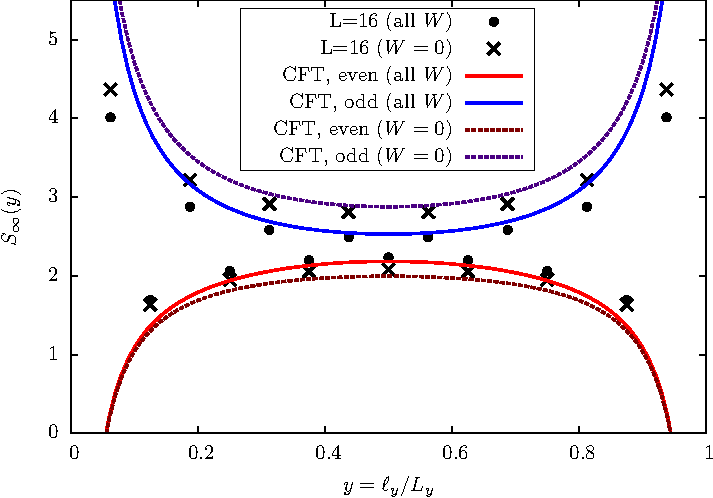
\includegraphics[width=8cm]{./figures/sinfty_16.pdf}
  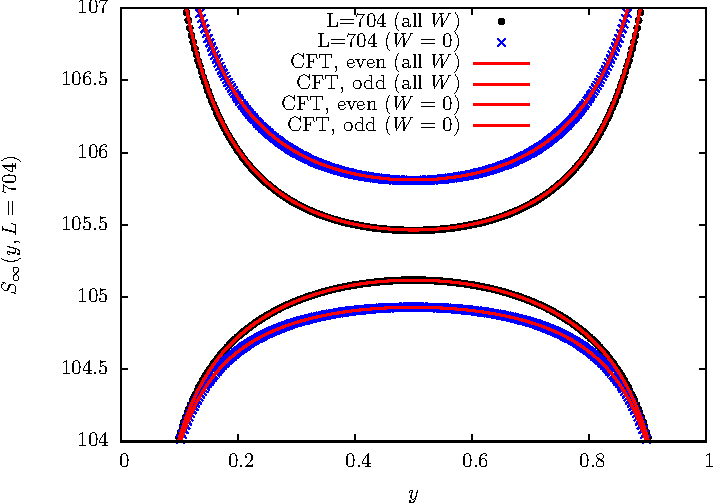
\includegraphics[width=8cm]{./figures/sinfty_704.pdf}
 \end{center}
\caption{Comparison numerics/analytics in the exactly solvable case $S_\infty$. Black points are the numerical data for the all sector, and blue crosses represents the numerical data in the $W=(0,0)$ sector. \emph{Left:} $L_x=16$, the data is compared with Eqs.~(\ref{eq:cft_prediction}) and (\ref{eq:cft_w0}) up to a single constant. The agreement is fair, but still far from converged. \emph{Right:} Same procedure for $L=704$. The agreement is perfect, as expected. }
\label{fig:Sinfty}
\end{figure}
\section{Entanglement in the $SU(N)$ RVB wave function}
\label{sec:rvb_entanglement}\paragraph{}
We now turn our attention to the $SU(N)$ RVB state, following the previous study\cite{Ju2012} of the $SU(2)$ case. First we remark that the Schmidt decomposition we performed for the quantum dimer model is not valid anymore, owing to the non-orthogonality of valence-bond states.
\paragraph{}
This section is organized as follows. In \ref{sec:su2_numerics} we recall the numerical result for the $SU(2)$ RVB state previously obtained in \cite{Ju2012}. We then present a simple CFT argument for the universal shape after the transition in \ref{sec:sun_cft}, before presenting our numerical result for the more general $SU(N)$ case (\ref{sec:sun_numerics}). We finally try in \ref{sec:extraction} to extract the exponent from the $SU(2)$ data, using the even-odd effect. Despite very strong finite-size effects, the result is compatible with CFT. 
\subsection{Numerical shape and even-odd effect for $SU(2)$}
\label{sec:su2_numerics}
We first begin with the $SU(2)$ case, and present the computation of $S_2$, and also $S_2$ restricted to the $W=(0,0)$ winding sector. The data is shown in Fig.~\ref{fig:SU2_shape}.
\begin{figure}[ht]
 \begin{center}
  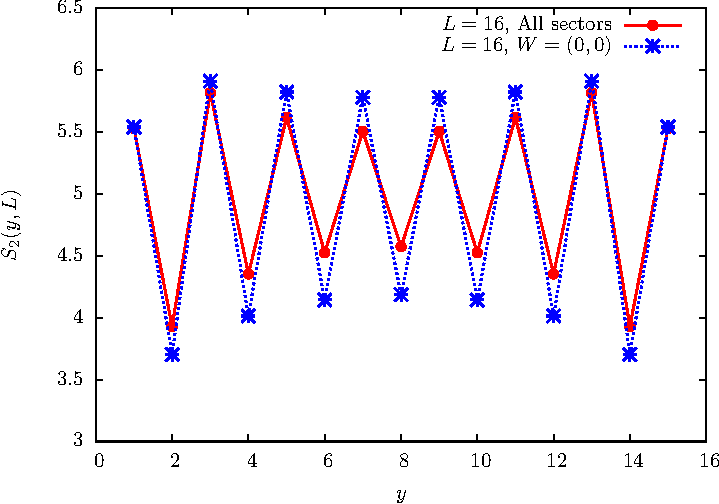
\includegraphics[width=8cm]{./figures/SU2_shape.pdf}
 \end{center}
\caption{Numerical extraction of the universal shape of $S_2$ as a function of $y=\ell_y/L_y$ for the $SU(2)$ RVB wave function (red solid lines). We also show the entropy in the zero winding sector (blue dotted lines), where the even odd effect is even stronger. }
\label{fig:SU2_shape}
\end{figure}
\paragraph{}We observe a striking similarity with the dimer data. In particular, the even-odd effect is bigger in the $W=(0,0)$ than in the ``all'' sector. Such a result is a strong evidence of universal behavior, and it is tempting to conclude that $S_2$ also lies in a locked phase. This is supported by the mapping to interacting dimers\cite{Damle} (which would predict $n_c= 2/\alpha\simeq 0.6$). We also performed exact diagonalizations on small systems, which show that the biggest eigenvalues of the RDM is non-degenerate (suggesting $d_{\rm min}=1$) as well as a big entanglement gap\footnote{Defining $\Delta=-\ln (p_1/p_{\rm max})$, we have the exact\cite{Stephan12,FisherStephenson} $\Delta_{\rm dimers}=2\ln \pi\simeq 2.29$ for dimers and $\Delta_{SU(2)}\approx 2.67$ for $SU(2)$ on a $4\times 4$ torus.}. 
\subsection{Universal shape from CFT}
\label{sec:sun_cft}
In the locked phase, we expect Eq.~(\ref{eq:shape_general}) to still be valid, but with a different $\alpha$ exponent. This is particularly useful because the problem once again reduces to a ratio of standard partition functions. Under the assumption that the conformal boundary conditions don't change compared to the dimers, we get 
\begin{eqnarray}\label{eq:cft_prediction_gen}
 s_n^{\rm (even)}(y,\tau)&=&\frac{n}{1-n}\ln \left(\frac{\alpha}{2}\times\frac{\eta(\tau)^2}{\theta_3(\alpha\tau)\theta_3(\tau/\alpha)}\times\frac{\theta_3(\alpha y \tau)\theta_3(\alpha(1-y)\tau)}{\eta(y\tau)\eta(2(1-y)\tau)}\right)\\
 s_n^{\rm (odd)}(y,\tau)&=&\frac{n}{1-n}\ln \left(\frac{\alpha}{2}\times\frac{\eta(\tau)^2}{\theta_3(\alpha\tau)\theta_3(\tau/\alpha)}\times\frac{\theta_4(2y \tau)\theta_4(2(1-y)\tau)}{\eta(2y\tau)\eta(2(1-y)\tau)}\right)
\end{eqnarray}
\begin{figure}[ht]
 \begin{center}
  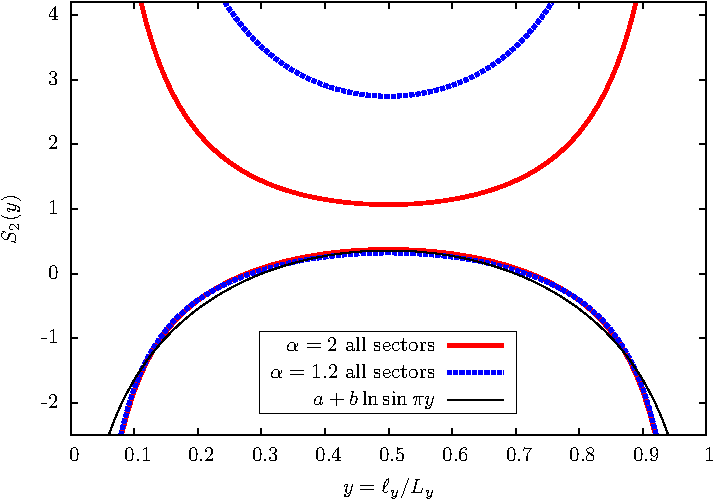
\includegraphics[width=8cm]{./figures/SUN_CFT.pdf}
 \end{center}
\caption{CFT prediction for the universal shape of $S_2$, as a function of $y=\ell_y/L_y$. Red solid lines correspond to the dimer model, with critical exponent $\alpha=2$. Blue dashed line is the $SU(2)$ RVB case, with exponent $\alpha\sim 1.2$. As emphasized in the text, it is very difficult to test this prediction with sufficiently accurate numerical precision.}
\label{fig:SUN_CFT}
\end{figure}
without restrictions on the winding numbers. To give an idea about the behavior of these functions, we plot them in Fig.~\ref{fig:SUN_CFT} for the two values of $\alpha$ corresponding to $SU(2)$ RVB and dimers. We observe that the shape (especially for the even branch) depends weakly on the exponent $\alpha$. Combined with the strong finite-size effects already mentioned, this makes an extraction of $\alpha$ from the numerical shape next to impossible. Notice however that the amplitude of the even-odd difference is much more pronounced for $\alpha=1.2$. We will use this fact in \ref{sec:extraction}, as a better method to extract $\alpha$ from the numerical data. 
\paragraph{}
Notice that also the prediction Eq.~(\ref{eq:cft_w0}) for the $W=(0,0)$ can be generalized:
\begin{eqnarray}\label{eq:cft_w0_gen}
 s_\infty^{\rm (even)}&=&-\ln \left(\frac{\alpha}{2}\frac{\eta(\tau)^2\theta_3(\alpha y(1-y)\tau)}{\eta(2y\tau)\eta(2(1-y)\tau)}\right)\\\label{eq:cft_w0_gen2}
 s_\infty^{\rm (odd )}&=&-\ln \left(\frac{\alpha}{2}\frac{\eta(\tau)^2\theta_4(\alpha y(1-y)\tau)}{\eta(2y\tau)\eta(2(1-y)\tau)}\right)
\end{eqnarray}
\subsection{Numerical results for $SU(N)$}
\label{sec:sun_numerics}
Before presenting the numerical results, an important point must be made: while we expected the $N\to \infty$ limit to correspond to dimers in terms of correlation functions, this is not at all obvious for the entanglement entropy. There are two reasons for this:
\begin{itemize}
 \item The Hilbert space corresponding to the $SU(N)$ RVB state is much bigger than that of the quantum dimer model. In particular, a singlet crossing the boundary would carry much more entropy than its dimer counterpart. Notice also that the RDM for $SU(N)$ has blocks with non-zero total spin, while these are by construction forbidden in the quantum dimer model.  
 \item One can reasonably expect this non-universal effects to only contribute to the area law term. It is however not clear in which phase $s_n(y,\tau,\alpha)$ will lie, since the critical parameter also depends on a non universal parameter, which is not very well defined for $SU(N)$.
\end{itemize}
The numerical results are shown in Fig.~\ref{fig:SUN_shape}
\begin{figure}[ht]
 \begin{center}
  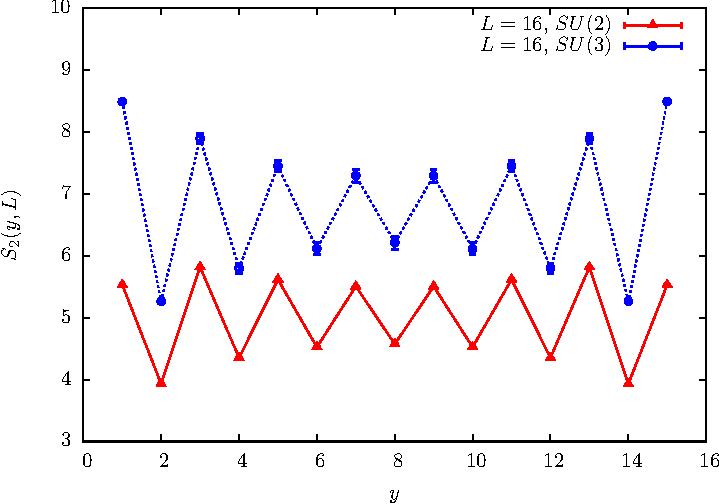
\includegraphics[width=8cm]{./figures/SUN_shape.pdf}
 \end{center}
\caption{Numerical data for the second R\'enyi entropy $S_2$ in the $SU(2,3,4,5)$ case. }
\label{fig:SUN_shape}
\end{figure}
\textcolor{red}{\bf [Waiting a bit for the $SU(4)$ and $SU(5)$ data to converge, since the conclusion should depend on the result.]}
\subsection{Extracting the critical exponent from the entanglement data}
\label{sec:extraction}
As already emphasized, the shape of the universal curve depends weakly on the critical exponent. 
Perhaps the best try to extract the critical exponent is to look at the even-odd difference for $y=1/2$. On the lattice it is defined as $\delta_n(L_x,L_y)=\left|S_n(L_y/2+1)-S_n(L_y/2)\right|$ for even $L_y$. This difference should go to a positive constant in the thermodynamic limit. From Eq.~(\ref{eq:cft_prediction_gen}) we predict
\begin{equation}\label{eq:even_odd}
 \delta_n(\tau,\alpha)=\frac{2n}{1-n}\ln \left(\frac{\theta_4(\alpha\tau/2)}{\theta_3(\alpha \tau/2)}\right)
\end{equation}
This allows in principle to determine the critical exponent from the entanglement data. Such an analysis is performed for quantum dimers as well as the $SU(2)$ RVB in Fig.~\ref{fig:evenodd}. As can be seen, finite-size effect again turn out to be very strong, even for quantum dimers. We observe the same kind of sublinear scaling for this quantity on small system sizes\cite{Ju2012}. However, as the $S_\infty$ data for quantum dimer can be rigorously shown to converge, it is reasonable to expect that the same happens for $S_2$.
\begin{figure}[ht]
\begin{center}
 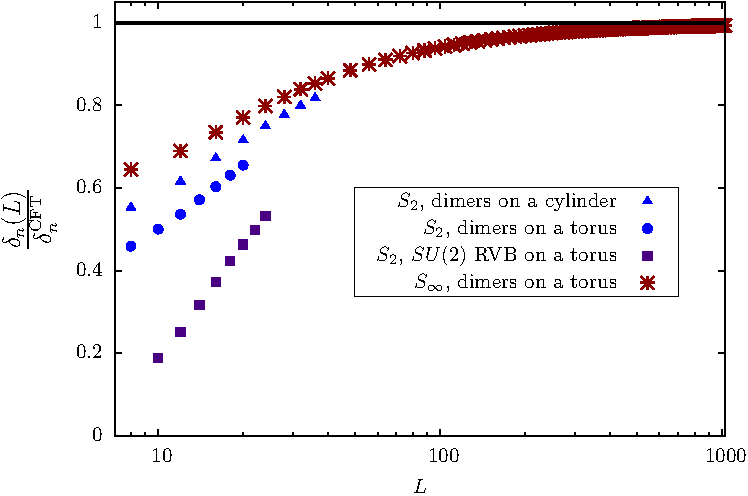
\includegraphics[width=8.1cm]{./figures/evenodd.pdf}
 %\hfill
 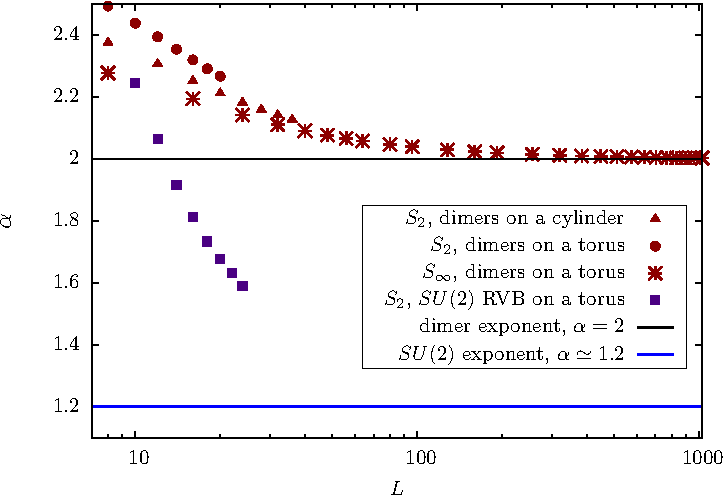
\includegraphics[width=8.1cm]{./figures/evenodd_alpha.pdf}
 \end{center}
 \caption{Even odd difference $\delta_n(L_x,L_y)=|S_n(L_x/2)-S_n(L_x/2-1)|$. \emph{Left Panel:} Convergence of $\delta_n(L)$ to the expected value from Eq.~(\ref{eq:even_odd}). \emph{Right Panel:} Finite-size extraction of $\alpha$ by solving $\delta_n(L_x,L_y)$ to Eq.~(\ref{eq:even_odd}). For quantum dimers as well as $SU(2)$, we observe an apparent sublinear scaling on small system sizes, which can be shown to go away for quantum dimers $S_\infty$.}
 \label{fig:evenodd}
\end{figure}
\section{Conclusion}
\label{sec:conclusion}
\textcolor{red}{\bf [To do]}
Study of $SU(N)$ RVB wave function:

\begin{itemize}
 \item Correlations: interpolation between $SU(2)$ and Quantum dimers. Monte-Carlo simulations. Critical exponents match those of Damle et al.
 \item Entanglement: more complicated observable. We observe universal aspects: Phase transition discussed in \cite{Stephan11}, even-odd effect. Shape should be universal. Strong finite-size effects.
 \item Regardless of the precise expression, the shape has to come from Coulomb gas, which means some function of $\alpha$, the geometry and the conformal boundary condition. The result will be close to \emph{not} $\ln \sin \pi y$, but \emph{not} exactly that. 
 \item Entanglement spectrum, $n \to \infty$ effectively cuts (at the level of universality) the system in 2 (exact on the lattice for dimers, quasi-exact on the lattice for RVB). 
 \item Difficulty to identify topological order for states that are also critical.
 \item Other ideas?
\end{itemize}

\paragraph{Acknowledgments}
 We would like to thank G. Misguich, V. Pasquier and \ldots \,for stimulating discussions. Grants. 
 \appendix
 \clearpage
\section{R\'enyi-Shannon entropy on the torus}
\label{sec:lgv}
We wish to compute the following classical entropy
\begin{equation}
 S_n=\frac{1}{1-n} \ln \left(\sum_{\sigma,\mu} [p_{\sigma,\mu}]^n\right), 
\end{equation}
for any real $n$. The probabilities $p_{\sigma,\mu}$ we are interested in are given by a ratio of partition functions, which can handily be expressed using a transfer matrix
\begin{equation}\label{eq:tm}
 p(\sigma,\mu)=\frac{Z_{\sigma.\mu}^A Z_{\mu,\sigma}^B}{Z}=\frac{\langle  \sigma|T^{\,\ell_y}|\mu\rangle\langle \mu|T^{\,L_y-\ell_y}|\sigma\rangle}{{\rm Tr}\; T^{L_y}}
\end{equation}
$T$ is the transfer matrix of the dimer model, and acts on the vector space generated by dimer occupancies on vertical edges along a horizontal line: $\langle a|T|b\rangle=1$ if configuration $|a\rangle$ and $|b\rangle$ are compatible, $0$ otherwise. The denominator is calculated in \ref{sec:dimers_exact}. Each factor on the numerator of Eq.~(\ref{eq:tm}) can be evaluated by a mapping onto free fermions\cite{Lieb1967,Alet_dimers2,Misguich}, as explained in Fig.~\ref{fig:freefermions}.  
\begin{figure}[ht]
\begin{center}
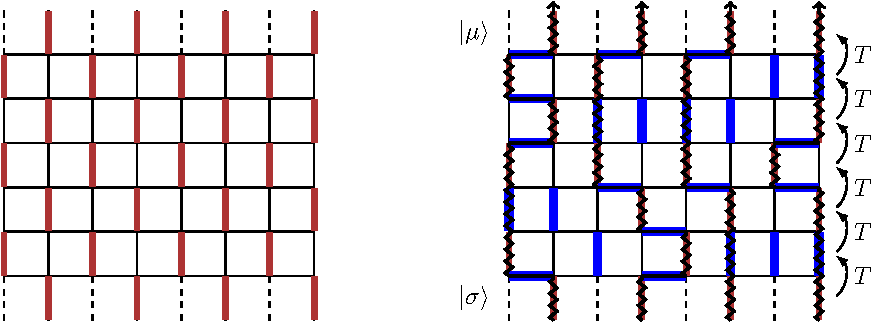
\includegraphics{./figures/free_fermions.pdf}
  \end{center}
  \caption{Illustration of the mapping onto free fermions. \emph{Left:} reference configuration with staggered dimers. \emph{Right:} transition graph generated by superimposing the reference configuration on the actual dimer configuration (in blue). This generates a collection of non-intersecting lattice paths, which can handily be expressed in terms of fermions. }
  \label{fig:freefermions}
  \end{figure}
A fermion is defined as an even vertical link occupied by a dimer, or an odd vertical empty link. $|\sigma\rangle$ and $|\mu\rangle$ can be rewritten in the antisymmetric fermionic basis
\begin{eqnarray}
|\sigma \rangle&=&|x_1,x_2,\ldots,x_N\rangle=c_{x_1}^\dag c_{x_2}^\dag \ldots c_{x_N}^\dag |0\rangle \\
|\mu \rangle&=&|y_1,y_2,\ldots,y_N\rangle=c_{y_1}^\dag c_{y_2}^\dag \ldots c_{y_N}^\dag |0\rangle
\end{eqnarray}
where the $x_i$ and $y_j$ label the ordered positions of the fermions. Introducing of shift of $+1$ lattice spacing from one row to the other, it is easy to check from Fig.~\ref{fig:freefermions} that the transfer matrix satisfies
\begin{eqnarray}
T|0\rangle&=&|0\rangle\\
T c_{2j}^\dag T^{-1}&=&c_{2j}^\dag+c_{2j+1}^\dag +c_{2j+2}^\dag\\
T c_{2j+1}^\dag T^{-1}&=&c_{2j+2}^\dag
\end{eqnarray}
Periodic boundary condition implies $c_{L_x}^\dag=(-1)^{N+1}c_0^\dag$. Writing this in matrix form using Einstein's summation convention
\begin{equation}
 T c_i^\dag T^{-1}=M_{ij} c_j^\dag,
\end{equation}
we successively get
\begin{equation}
 T^\ell c_i^\dag T^{-\ell}=\left(M^\ell\right)_{ij} c_j^\dag
\end{equation}
and 
\begin{eqnarray}
\langle \sigma |T^\ell |\mu\rangle&=&\langle 0|c_{x_1} c_{x_2} \ldots c_{x_N} T^{\ell} c_{y_1}^\dag c_{y_2}^\dag \ldots c_{y_N}^\dag |0\rangle \\ 
&=&\langle 0|c_{x_1} c_{x_2} \ldots c_{x_N} (M^\ell)_{y_1 z_1}c_{z_1}^\dag (M^\ell)_{y_2 z_2}c_{z_2}^\dag \ldots (M^\ell)_{y_N z_N}c_{z_N}^\dag|0\rangle
\end{eqnarray}
By applying the Wick's theorem and using $\langle 0|c_x c_y^\dag|0\rangle=\delta_{xy}$, we finally get
\begin{equation}
 \langle \sigma |T^\ell |\mu\rangle=\det_{1\leq i,j\leq N} \left[(M^\ell)_{x_i y_j}\right]
\end{equation}
This result is nothing but Lindstr\"om-Gessel-Viennot\cite{Lindstrom1973,GesselViennot1989} lemna applied to the non intersecting lattice paths generated by dimers. In the end, Eq.~(\ref{eq:tm}) reduces to a product of two determinants. 
\section{CFT correlations and partition functions}
\label{sec:CFT_Jacobi}
\subsection{Dedekind-eta and Jacobi-Theta functions}
For a given modulus $\tau=i L_y/L_x$, we introduce the squared nome:
\begin{equation}
 q=e^{2i\pi \tau}=e^{-2\pi L_y/L_x}
\end{equation}
The Dedekind eta function is defined as 
\begin{equation}
 \eta(\tau)=q^{1/ 24}\prod_{k=1}^{\infty}\left(1-q^k\right),
\end{equation}
and the four Jacobi Theta functions are given by
\begin{eqnarray}
 \theta_1(z|\tau)&=&\sum_{n \in \mathbb{Z}}(-1)^{n-1/2}q^{\frac{1}{2}(n+1/2)^2}e^{(2n+1)iz}\\
 &=&2\eta(\tau)q^{1/6} \sin z\prod_{n=1}^{\infty} \left[1-2 \cos(2z) q^{n}+q^{2n}\right]
\end{eqnarray}
\begin{eqnarray}
 \theta_2(z|\tau)&=&\sum_{n \in \mathbb{Z}}q^{\frac{1}{2}(n+1/2)^2}e^{(2n+1)iz}\\
 &=&2\eta(\tau)q^{1/6} \cos z\prod_{n=1}^{\infty} \left[1+2 \cos(2z) q^{n}+q^{2n}\right]
\end{eqnarray}
\begin{eqnarray}
 \theta_3(z|\tau)&=&\sum_{n \in \mathbb{Z}}q^{\frac{1}{2}n^2}e^{2niz}\\
 &=&\eta(\tau)q^{-1/12}\prod_{n=1}^{\infty} \left[1+2 \cos(2z) q^{n-1/2}+q^{2n-1}\right]
\end{eqnarray}
\begin{eqnarray}
 \theta_4(z|\tau)&=&\sum_{n \in \mathbb{Z}}(-1)^{n}q^{\frac{1}{2}n^2}e^{2niz}\\
 &=&\eta(\tau)q^{-1/12}\prod_{n=1}^{\infty} \left[1-2 \cos(2z) q^{n-1/2}+q^{2n-1}\right]
\end{eqnarray}
To simplify the notations a bit, we also set
\begin{equation}
 \theta_\nu(\tau)=\theta_\nu (0|\tau)\quad,\quad \nu=1,2,3,4
\end{equation}
\subsection{Modular transformations}
\label{sec:modular}
All these functions obey the following nice transformation properties. 
\begin{eqnarray}
 \theta_1(\tau)&=&-i (-i \tau )^{-1/2}\,\theta_1(-1/\tau)\\
 \theta_2(\tau)&=&(-i \tau )^{-1/2}\,\theta_4(-1/\tau)\\
 \theta_3(\tau)&=&(-i \tau )^{-1/2}\,\theta_3(-1/\tau)\\
 \theta_4(\tau)&=&(-i \tau )^{-1/2}\,\theta_2(-1/\tau)\\
 \eta(\tau)&=&(-i \tau )^{-1/2}\,\eta(-1/\tau)
\end{eqnarray}
\subsection{Partition functions in various geometries for the free boson}
Here $\tau=iL_y/L_x$, for a cylinder of circumference $L_x$ and height $L_y$. The calculation of partition function in torus and cylinder with various boundary condition is standard, see for example\cite{EggertAffleck,FSW,BigYellowBook}. We list some of them below.
\begin{itemize}
 \item Cylinder with Dirichlet boundary condition at both ends:
 \begin{equation}\label{eq:cylinder_dd}
 \mathcal{Z}_{\rm cyl}^{DD}=g_{D}^2 \,\frac{\theta_3(\alpha \tau)}{\eta(2\tau)}
\end{equation}
\item Cylinder with the shifted boundary condition discussed in the text:
\begin{equation}\label{eq:cylinder_ddprime}
 \mathcal{Z}_{\rm cyl}^{DD^\prime}=g_{D}^2 \,\frac{\theta_4(\alpha \tau)}{\eta(2\tau)}
\end{equation}
\item Cylinder with Neuman at one end, and Dirichlet at the other:
\begin{equation}
 {\cal Z}_{\rm cyl}^{ND}=g_N g_D \, \frac{\theta_4(4\tau)}{\eta(2\tau)}
\end{equation}
\item Torus partition function
\begin{equation}
 {\cal Z}_{\rm torus}=\frac{\theta_3(\alpha \tau)\theta_3(\tau /\alpha)}{\eta(\tau)^2}
\end{equation}
\end{itemize}
$g_D$ and $g_N$ are the universal Affleck-Ludwig\cite{AffleckAndLudwig,FSW} g-factors, corresponding to the Dirichlet and Neuman boundary condition.
\begin{eqnarray}
 g_D&=& (\alpha/2)^{1/4}\\
 g_N&=& (2\alpha)^{-1/4}
\end{eqnarray}
\section{Derivation of CFT partition function from the lattice dimer model}
\label{sec:dimers_exact}
\subsection{Torus}
The goal of this section is to recover the CFT partition function on the torus, using the exact solution for dimers in terms of transfer matrix, and keeping track of the winding numbers $W_x$ and $W_y$. To do that we need to solve a slightly more complicated problem than that in \ref{sec:lgv}, introducing a fugacity $b$ (resp. $b^{-1}$) for horizontal dimers whose left site belongs to the even (resp. odd) sublattice. We will also suppose $L_x$ and $L_y$ to be even. With this at hand the transfer matrix now satisfies
\begin{eqnarray}
T|0\rangle&=&|0\rangle\\
T c_{2j}^\dag T^{-1}&=&b \,c_{2j}^\dag+c_{2j+1}^\dag +b^{-1}c_{2j+2}^\dag\\
T c_{2j+1}^\dag T^{-1}&=&c_{2j+2}^\dag
\end{eqnarray}
The $b$'s provide information about $W_x$, while the number of fermions does that for $W_y$. 
Defining as before $T c_i^\dag T^{-1}=M_{ij} c_j^\dag$, diagonalizing $T$ amounts to diagonalizing $M$, which can be done in Fourier space, carefully taking into account the boundary condition on fermions
\begin{equation}
 c_{L_x}^\dag=(-1)^{\hat{N}+1}c_0^\dag\quad,\quad \hat{N}=\sum_{j=1}^{L_x} c^\dag_j c_j
\end{equation}
We write the number of dimer coverings in the $(W_x,W_y)$ sector as $Z_{W_x,W_y}$. Setting $b=e^{-\pi u_x/L_x}$, the winding generating function is given by
\begin{eqnarray}
 Z(u_x,u_y)&=&\sum_{W_x,W_y} Z_{W_x,W_y}e^{-\pi (W_x u_x+W_y u_y)}\\\label{eq:Z_tm}
 &=&{\rm Tr}\left[\displaystyle{e^{-\pi u_y(\hat{N}-L_x/2)/2}T^{L_y}}\right]
\end{eqnarray}
If we now denote by $d_k^\dag$ the set of fermionic operators that diagonalize the one-particle transfer matrix
\begin{equation}
 T d_k^\dag T^{-1}=\lambda_k d_k^\dag,
\end{equation}
the $\lambda_k$ are then the eigenvalues of $M$. Using this, the transfer matrix can be expressed as
\begin{equation}
 T=\prod_k \left(1+[\lambda_k -1]d_k^\dag d_k \right)
\end{equation}
Plugging this expression in Eq.~(\ref{eq:Z_tm}) we get\footnote{One can check easily that expanding simultaneously the first two product in Eq.~(\ref{eq:dimers_torus}) generates all the eigenvalues of the transfer matrix in the even fermion sector. The same goes for the last two products and the odd-fermions sector. }
\begin{eqnarray}\nonumber
 Z(u_x,u_y)&=&\prod_{k\in \Omega_{1}}\left[e^{\pi x /2}+e^{-\pi x/2}\lambda_k^{L_y}\right]+\prod_{k\in \Omega_{1}}\left[e^{\pi x/2}-e^{-\pi x/2}\lambda_k^{L_y}\right]\\\label{eq:dimers_torus}
 &+&\prod_{k\in \Omega_{0}}\left[e^{\pi x /2}+e^{-\pi x/2}\lambda_k^{L_y}\right]-\prod_{k\in \Omega_{0}}\left[e^{\pi x /2}-e^{-\pi x/2}\lambda_k^{L_y}\right]
\end{eqnarray}
with
\begin{eqnarray}
 \lambda_k&=&\cos k +\sqrt{1+\cos^2 k}\\
\Omega_{\nu}&=&\left\{\frac{(2m+\nu+i u_y) \pi}{L_x}\quad,\quad m=-L_x/2,\ldots,L_x/2-1\right\} 
\end{eqnarray}
Of course, $Z(u_x=0,u_y=0)$ reduces to the well known torus partition function obtained by Kasteleyn and Fisher. 
\paragraph{}We now wish to extract the universal CFT partition function $\mathcal{Z}$, i.e the constant term in the asymptotic expansion of $Z$:
\begin{equation}
 Z(u_x,u_y)\sim A^{L_x L_y} B^{L_x} C^{L_y}\mathcal{Z}(u_x,u_y)
\end{equation}
A possible way to do so would be to combine Euler-Maclaurin expansions and majoration techniques, as has already been done for the honeycomb lattice\cite{Boutillier}. Here we obtain $\mathcal{Z}$ in a more heuristic (and non rigorous) manner, noticing that universal properties have to come from low energy excitation near the Fermi momenta $k_F=\pm \pi/2$. Linearizing $\ln(\lambda_k)$ around the two $k_F$ and extending the products in \ref{eq:dimers_torus} over all integers, allows to go get after a long calculation, very similar to that in \cite{Boutillier}:
\begin{equation}
 \mathcal{Z}(u_x,u_y)=\frac{\displaystyle{\theta_3(i\pi u_x/2|\tilde{\tau}/2)\,\theta_3(i\pi u_y/2|\tau/2)}}{\displaystyle{(2 \Im{\rm m}\, \tau)^{1/2}\,\eta(\tau)^2}}
\end{equation}
where $\tau=i L_y/L_x$ and $\tilde{\tau}=-1/\tau=iL_x/L_y$. 
\subsection{Cylinder}
The cylinder geometry is slightly simpler than its torus counterpart, because only the windings along $y$ are allowed. To still express the partition function as a trace, we look at the transfer matrix $\tilde{T}$ acting on the configuration of rows of length $L_y$ with \emph{open} boundary conditions. This way, the number of fermions keeps track of the winding number $W_y$. The winding generating function can be expressed, after some algebra, as
\begin{eqnarray}
 Z(u_y)&=&e^{-\pi (L_y/2)u_y}\prod_{m=1}^{L_y} \left(1+e^{\pi u_y}\mu_m^{L_x}\right)\\
 \mu_m&=&\cos \left(\frac{m \pi}{L_y+1}\right)+\sqrt{1+\cos^2\left(\frac{m \pi}{L_y+1}\right)}
\end{eqnarray}
Here the Fermi momentum is $k_F=\pi/2$, and the CFT partition function can be accessed using the linearization trick. We, however have to distinguish between the even and odd $L_y$ cases.
\paragraph{Even case}
It is most convenient to rewrite $Z$ as
\begin{equation}
Z(u_y)=\prod_{m=1}^{L_y/2} \lambda_m^{L_x}\times \left[\prod_{m=1}^{L_y/2} 1+2\cosh (\pi u_y)\mu_m^{-L_x}+\mu_m^{-2L_x}\right] 
\end{equation}
Combining the Euler-Maclaurin formula on the first product, and using the linearization procedure around $m=L_y/2$, we get
\begin{equation}
 \mathcal{Z}= e^{\frac{\pi L_x}{24 L_y}}\prod_{p=1}^{\infty}\left[1+2 \cosh (\pi u_y)e^{-\frac{\pi L_x}{L_y}(p-1/2)}+e^{-2\frac{\pi L_x}{L_y}(p-1/2)}\right]
\end{equation}
which gives, using the infinite product representation of the Jacobi Theta function,
\begin{equation}
 \mathcal{Z}=\frac{\theta_3(i \pi u_y/2|\tilde{\tau}/2)}{\eta(\tilde{\tau}/2)}
\end{equation}
We recover the CFT result (\ref{eq:cylinder_dd}), upon setting $u_y=0$ and performing a modular transformation. 
\paragraph{Odd case}
We use the same method, but care must be taken because of the presence of a zero-mode for $m=(L_y+1)/2$ We have
\begin{equation}
Z(u_y)=2\cosh(\pi u_y/2)\prod_{m=1}^{(L_y-1)/2} \lambda_m^{L_x}\times \left[\prod_{m=1}^{(L_y-1)/2} 1+2\cosh (\pi u_y)\mu_m^{L_x}+\mu_m^{2L_x}\right] 
\end{equation}
which yields after linearization
\begin{equation}
 \mathcal{Z}= 2 e^{-\frac{\pi L_x}{12 L_y}}\cosh(\pi u_y/2)\prod_{p=1}^{\infty}\left[1+2 \cosh (\pi u_y)e^{-\frac{\pi L_x}{L_y}p}+e^{-2\frac{\pi L_x}{L_y}p}\right]
\end{equation}
In the end we obtain:
\begin{equation}
 \mathcal{Z}=\frac{\theta_2(i \pi u_y/2|\tilde{\tau}/2)}{\eta(\tilde{\tau}/2)}
\end{equation}
and once again recover the CFT result (\ref{eq:cylinder_ddprime}) after setting $u_y=0$ and modular transformation. 
\subsection{Zero-winding sectors}
With the winding generating function at hand, the calculation of $s_n(y,\tau)$ in the $W=(0,0)$ winding sector becomes straightforward. For example we have (recall $\tau=iL_y/L_x$ and $\tilde{\tau}=-1/\tau$)
\begin{eqnarray}\label{eq:nullwinding1}
\underbrace{\mathcal{Z}_{\rm cyl}^{DD^\prime}(y\tau)\mathcal{Z}_{\rm cyl}^{DD^\prime}((1-y)\tau)}_{W=(0,0)}&=&\frac{1}{\eta(\frac{\tilde{\tau}}{2y})\eta(\frac{\tilde{\tau}}{2(1-y)})} 
\underbrace{\theta_2\left(\frac{i \pi u_y}{2}\right.\left|\frac{\tilde{\tau}}{2y}\right)\theta_2\left(\frac{i \pi u_y}{2}\right.\left|\frac{\tilde{\tau}}{2(1-y)}\right)}_{W=(0,0)}\\\label{eq:nullwinding2}
&=&\frac{\theta_2\Big(0\left|\frac{\tilde{\tau}}{2y(1-y)}\right)}{\eta(\frac{\tilde{\tau}}{2y})\eta(\frac{\tilde{\tau}}{2(1-y)})}
\end{eqnarray}
Eq.~(\ref{eq:nullwinding2}) follows from Eq.~(\ref{eq:nullwinding1}) by selecting the term in $(u_y)^0$ in the product of theta functions. This allows to recover Eq.~(\ref{eq:cft_w0_gen}) and Eq.~(\ref{eq:cft_w0_gen2}) after once again a modular transformation. 
 \section*{References}
\bibliography{rvb2_bib.bib}{}
\bibliographystyle{unsrt}
\end{document}
